\setcounter{chapter}{5}
\setcounter{rq}{1}


\chapter{Evaluating Text Automatically Identified}
\label{ch:assisting}



In a previous chapter, we have shown that semantic-based techniques can identify part of the text 
that human annotators deemed relevant to a number of artifacts associated with Android tasks.
This however, does not address whether the text automatically identified assists a software developer
 in completing her task.



To shorten this gap, this chapter presents a \textit{controlled experiment} 
where we evaluate how developers complete software tasks when assisted, or not, by a tool that 
embeds one of our semantic-based techniques. 
We use three software tasks related to well-known Python modules and
report what text \red{12} developers deemed relevant to a first tasks they completed
as well as the developers' perception on the usefulness of text automatically
identified by our tool in a second task also completed by them. 


We start by describing experimental procedures (Section~\ref{cp6:procedures}) and then by presenting the results of our experiment (Section~\ref{cp6:results}). Section~\ref{cp6:summary} summarizes our key findings.



\clearpage

\section{Experimental Setup}
\label{cp6:procedures}



\gm{You need to provide the overall
design first. Hard to understand why
the tasks are as they are. More "Design' up-front.}


To determine how a tool embedding a semantic-based technique might assist developers complete a software task, we question whether:



\begin{enumerate}
    \item \textit{a developer would produce a more correct solution when assisted by such a tool;}
    \item \textit{the text automatically identified by the tool as potentially relevant to a task in a software artifact pertinent to that task is similar to text that developers would deem relevant; and if}
    \item \textit{a developer finds that the text automatically identified by the tool in an artifact under inspection assists her towards task completion.}
\end{enumerate}



To investigate these questions, we designed an experiment where participants attempted two programming
 using (or not) a tool that applies the \texttt{BERT} technique (Section~\ref{cp5:approach-bert})
 to  identify task-relevant text in the artifacts that were available to a participant in each task---highlighting the text automatically identified by the semantic-based technique in these artifacts. 


For each task, we compare solutions  submitted by participants who did, or did not, use the tool to assist them in that task. 
For that, we run a set of test cases that evaluate the correctness of the submitted solutions, what helps us answer RQ1.


In the tasks that participants performed without tool support, we asked them to manually indicate in the artifacts available for that task the text that they deemed useful for that task.
We use the manually provided text to investigate RQ2, analyzing to which extent our tool identifies the same text for that task.


We also asked participants to indicate how useful were the highlights shown in each of the artifacts available in the tool-assisted task
and prompted them to provide any additional feedback that they wished to share about the tool or the experiment (RQ3).






We detail experimental procedures in the following subsections.






% Our experiment's main hypothesis is that:


% \medskip
% \begin{bluequote}
%     \textit{text automatically identified by a semantic-based technique assists a 
%     developer complete her software development task.} 
% \end{bluequote}



% To test this hypothesis, 
 
%  \gm{Setting this up as a test of
%  a hypothesis sets a high bar where
%  there will be expectations of
%  refuting a null hypothesis. Is that
%  where you want to go?}

% %  For each of these tasks, we provided to the participants a curated list of natural language artifacts related to the task
% % and we asked them to code a solution for the task.
 
 
% %  when assisted (or not) by a
% %  tool that embeds one of the semantic-based techniques that we have explored previously ({Section~\ref{cp5:results-all}). 

% \gm{You need to provide the overall
% design first. Hard to understand why
% the tasks are as they are. More "Design' up-front.}

% In a first task, a participant manually identifies text relevant to that task (while performing the task)
% in a set of curated artifacts containing information that could assist the participant complete the task at hand.
% With this first task, we evaluate how the text that a participant manually identified as relevant
% compares to the text that an automatic technique would identify for that same task. 



% In a second task, each artifact associated to the task has a set of highlighted sentences. These 
% sentences represent text that an automatic approach ({Section~\ref{cp5:results-all}) identified as potentially useful for that task. 
% We ask a participant to indicate whether the highlights shown helped her complete their task.
% Hence, with this second task, we evaluate what is the participants' perceived usefulness of the text automatically identified.





% % \art{Add a figure to help summarizing the experimental setup?}



% \art{say somewhere that the experiment was performed remotely and without the researcher's assistance. }


\subsection{Design}


The experiment's independent variable represents the task configuration, i.e., if a participant had to manually indicated what text they deemed relevant to a task
or if our tool automatically did this step. We refer to these two configurations as \textit{manual} or \textit{tool-assisted}. 


Based on our independent variable, we follow a \textit{within-subjects} design. Each participant is exposed to exactly one manual task and one tool-assisted task.
We assigned tasks to a participant randomly. Nonetheless,  
we ensured that each task configuration (manual or tool-assisted) was seen by an equal number participants.
\gm{how is this design within-subjects?
Aren't you comparing across
the tasks which means across subjects?}








\subsection{Tasks}
\label{sec:experiment-tasks}



We expect the experiment to be executed offline, i.e., the experiment has self-contained instructions that allow a participant to perform their assigned tasks without any supervision.
\gm{Why not just say the participants
completed the tasks on their own time?}
This requires tasks that are easy to understand and perform in a single experimental session. At the same time, our main hypothesis requires tasks for which a developer will likely benefit from the use of additional information to complete.


These criteria lead us to select Python w3resource tasks\footnote{\url{https://www.w3resource.com/python-exercises/}}
that required usage of at least one module external to the Python core modules~\cite{thiselton2019}.
By using an external module, we aim to reduce the likelihood that a participant 
can provide a solution for a task without consulting any of the artifacts accompanying that task. 






Table~\ref{tbl:python-tasks-modules} details the tasks that we have selected. 
We chose these tasks due to how they focus on modules widely adopted both by open source systems and by private companies.
For example, the \texttt{NYTimes} task involves using a HTML parser, namely \texttt{BeautifulSoup},
which Reddit---a social news aggregator with approximately 430 million monthly users---uses 
to parse urls and identify images shown on its posts' headlines~\cite{bs4-reddit}. 
Similarly, the \texttt{Titanic} task encompasses using \texttt{Pandas}, a data analysis and manipulation module
used in many open source data science projects~\cite{ma2017, shrestha2020}.





\begin{table}
\centering
\caption{Python tasks}
\begin{footnotesize}
\rowcolors{2}{}{lightgray}
\begin{tabular}{ll}
\hline
\textbf{Task} & \textbf{Description}                                                                                         \\
\hline
\hline
%
\parbox[l][1cm][c]{1cm}{Practice task}       &
\parbox[l][1cm][c]{11cm}{Given three dictionaries representing address books,
you must write an algorithm using the Python core \texttt{dict} module to merge them.}    \\
\hline
%
Distances     &
\parbox[l][1.3cm][c]{11cm}{Given a string representing a rendezvou point and a list of suggested picnic addresses
    you must write an algorithm using the \texttt{geopy} module to find the  picnic address closest to the rendezvou point.} \\
%
NYTimes       &
\parbox[l][1cm][c]{11cm}{Given a string representing the url for NY Times Today's,
    write an algorithm using the \texttt{BeautifulSoup} and \texttt{requests} modules to scrape all the headlines of that page.}
\\
%
Titanic       &
\parbox[l][1cm][c]{11cm}{Given a string representing a url for the titanic dataset,
    you must write an algorithm using the \texttt{pandas} and \texttt{seaborn} modules to create a barchart of the data.}    \\
    
\hline
\end{tabular}
\end{footnotesize}
% \smallskip
\label{tbl:python-tasks-modules}
\end{table}









\subsection{Artifacts}
\label{sec:experiment-artifacts}


Each task requires a set of artifacts that a participant could peruse for information that could assist them complete the task.
We select artifacts for a task following procedures similar to the ones we used to create the \acs{DS-android} dataset (Chapter~\ref{ch:android-corpus}). 
For each of the tasks in Table~\ref{tbl:python-tasks-modules}, we use the Google search engine to obtain up to ten artifacts that likely contain relevant
information for that task. 






\subsection{Participants}



We advertised our study to both developers in our professional network and to computer science students at the several universities. 
This provides for breadth of experience where both novice and expert developers attempt the tasks in our experiment. 


With regards to computer science students, we sent the study only to third and fourth-year students to ensure that they had the necessary background required to perform the study's taks.
At this point in the curriculum, students should be familiar with Python and they should be able to come up with a solution 
for a software task when provided with artifacts containing information for that task.


To compensate participants for their time, we offered them the opportunity to enter a raffle for one of two iPads 64 GB.






\subsection{Procedures}
\label{cp6:evaluation-procedures}



The experiment was completely offline, i.e., it could be performed at a participant's personal computer
without the presence of one of the researchers. Each participant had to complete a practice task---separated from the experimental tasks---and two tasks (manual and tool-assisted) drawn from the tasks in Table~\ref{tbl:python-tasks-modules}. 


Each experimental session lasted no more than two hours; this length of time was selected based on two pilot sessions. 
Feedback from these pilots also helped to refine the experiment's instructions, where we included a short video showing how to install the web browser plugin and how to use Colab, the online environment where participants performed each task (Section~\ref{cp6:environment}).






We began each session gathering consent and requesting participants to install a web browser plugin which we used to gather data.
Setup was followed by a short tutorial explaining the experiment and describing how to use the plugin and Colab. 
The practice task allowed participants to familiarize themselves with the content of a task, the web browser plugin and Colab. 



For each task, including the practice tasks, we asked a participant to write a solution for the task
when provided with a fixed set of artifacts, e.g., official API documentation, Stack Overflow posts, or web tutorials, 
associated with that task.  


In the control task, a participant was instructed to use the web browser plugin to highlight any text that they deemed relevant to the task-at-hand. 
\gm{Do they highlight text as they
work or after the task?}
In the tool assisted task, the plugin automatically highlighted sentences that our semantic-based technique identified as relevant for the task. 
For this second task, we had one extra step asking the participant to rate---using a Likert scale---how helpful were the highlights automatically identified per artifact available. 
\gm{More detail about exactly
what participants were asked to
do and experimental materials
should be published or in Appendix
of thesis.}


We concluded the study by asking participants if they would like to provide any additional information and 
by giving them the opportunity to join the raffle, if so they wished. 



% \subsubsection{Summary of procedures}

% Based on our experimental procedures, we could gather:



% \begin{enumerate}
%     \item a participant's submitted solution (written Python code) for each task;
%     \item a participant's highlights for the control task; 
%     \item a participant's perception on the usefulness of the automatically identified highlights for the tool assisted task, and;
%     \item any additional feedback (written text) that a participant wished to provide us.
% \end{enumerate}




\subsection{Colab}
\label{cp6:environment}


To ensure that participants had the same conditions to perform each task
and also to minimize setup instructions, we used Google Colab\footnote{\url{https://colab.research.google.com/}} as our coding environment. 
% By using Colab, we also expect setup instructions to be minimal 
% so that we allow a participant to focus on the task and experimental procedures.



Figure~\ref{fig:nytimes-task-colab} shows an example of our online environment for the \texttt{NYTimes} task.
At the left-hand side, participants had the task description and examples of input and output scenarios as well as a list of resources associated with that task. 
By clicking on the coding environment link, participants were redirected to Colab (right-hand side),
where they had a code editor with amenities commonly found in modern IDEs, such as code completion and syntax highlighting. 



Through Colab, a participant could compile their solution and test it against the examples shown alongside the task description.
Upon testing, the system would display full details about the test cases, e.g., the test's input, which assertion failed, and why. 




\clearpage

\begin{landscape}
\begin{figure}
    \centering
    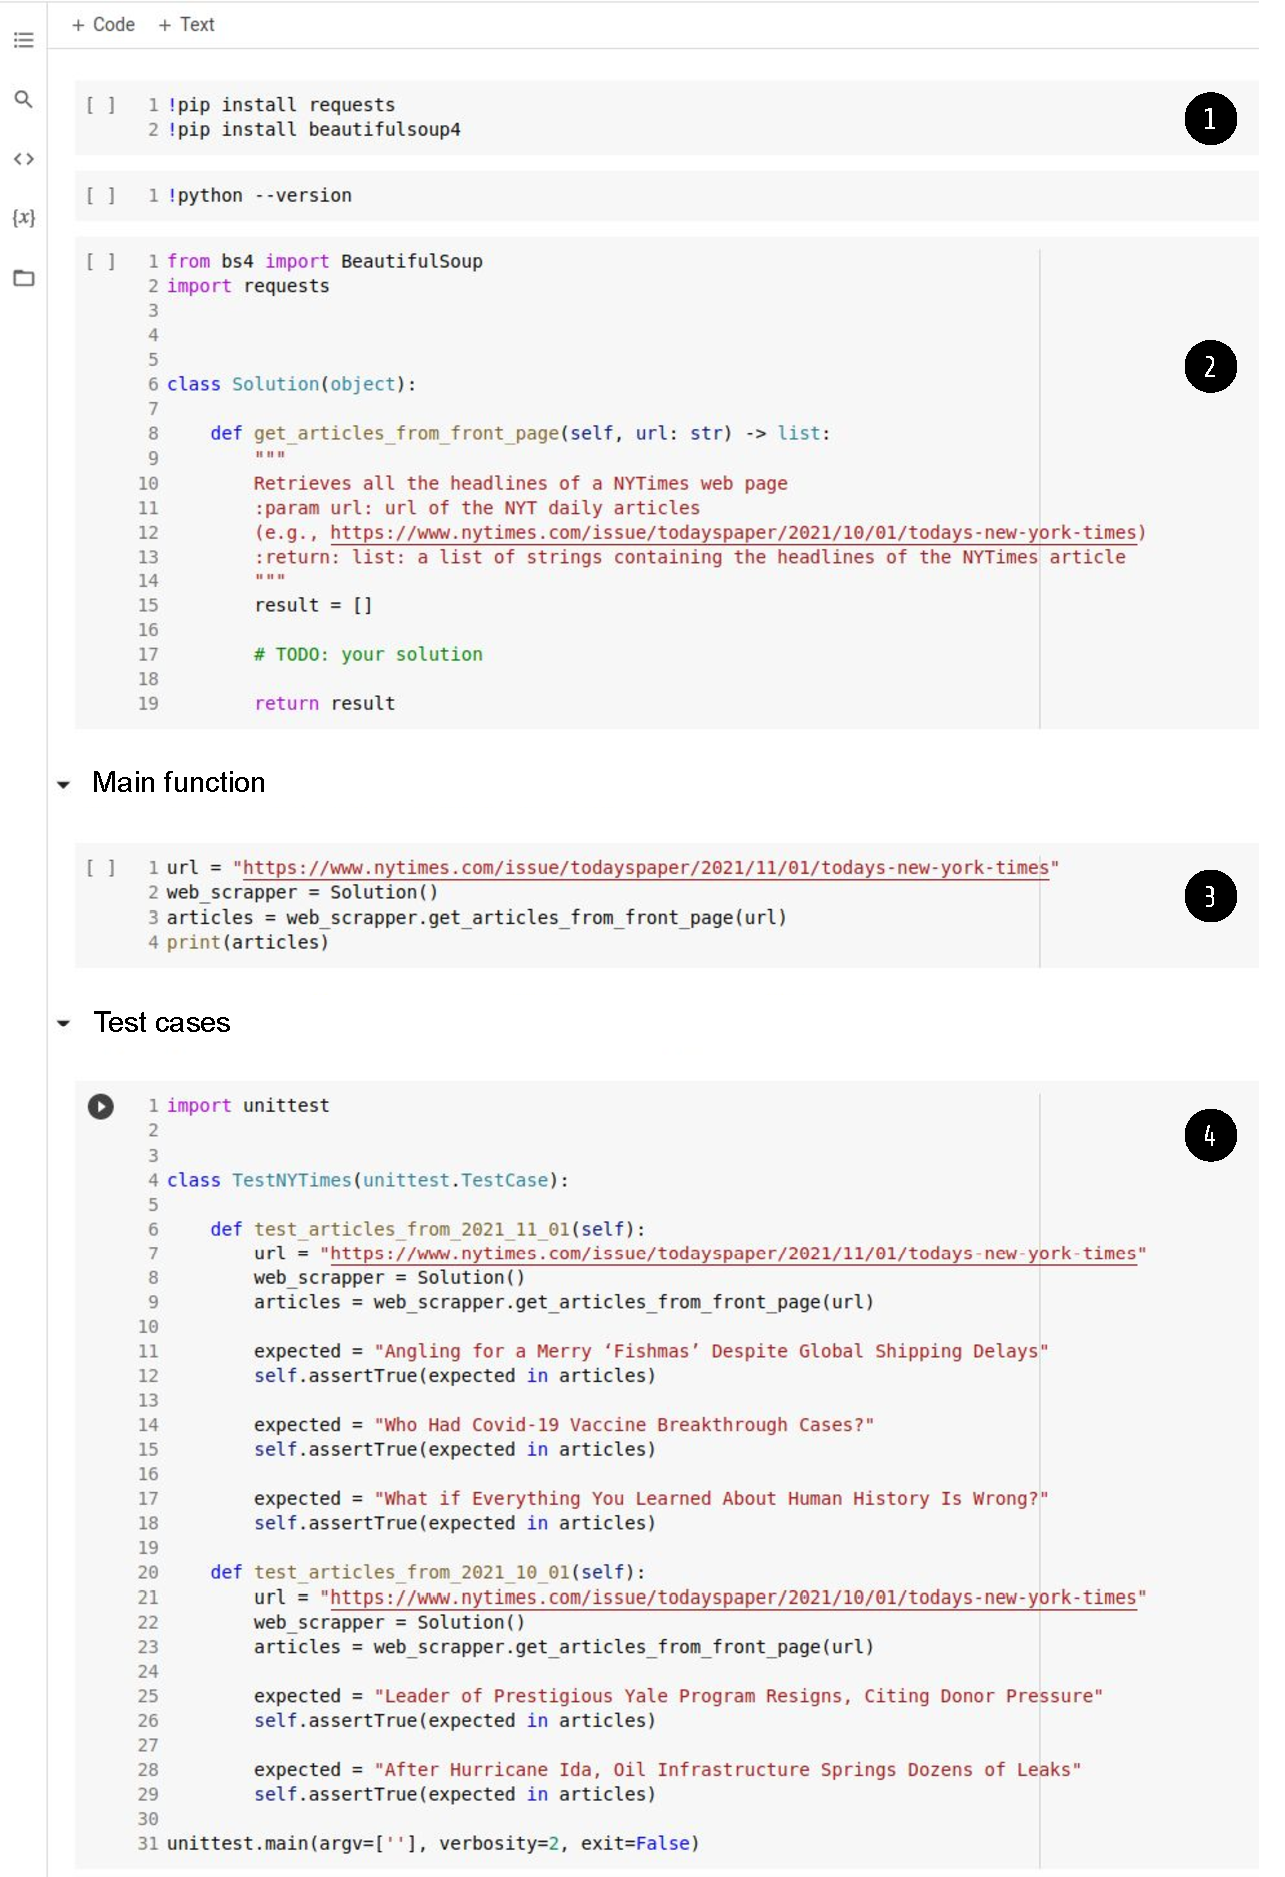
\includegraphics[width=1.5\textwidth]{cp6/task-colab.pdf}
    \caption{NYTimes task and Colab environment.}
    \label{fig:nytimes-task-colab}
\end{figure}
\end{landscape}

\clearpage


\subsection{Analysis}



Table~\ref{tbl:experiment-data} summarizes the data we collected based on experimental procedures.
We use the gathered data to investigate our main hypotheses according to the following metrics.



\begin{table}
\caption{Data collected}
\begin{small}
\vspace{-1mm}  


\begin{threeparttable}    
\rowcolors{2}{}{lightgray}
\begin{tabular}{ll}
\hline    
\textbf{} & \textbf{Data collected}  \\ 
\hline
\hline
1 & 
\parbox[l][0.8cm][c]{11cm}{
    participant's submitted solution (written Python code) for each task
}  
\\
%
2 & 
\parbox[l][0.8cm][c]{11cm}{
     participant's highlights for the control task
}  \\
3 & 
\parbox[l][1cm][c]{11cm}{
    a participant's perception on the usefulness of the automatically identified highlights for the tool assisted task
}  \\
4 & 
\parbox[l][0.8cm][c]{11cm}{
    any additional feedback (written text) that a participant wished to provide us
}  \\
\hline
\end{tabular}
\end{threeparttable}    
\end{small}
\smallskip
\label{tbl:experiment-data}
\end{table}
    



\subsubsection{Submitted Solution}

 
The correctness of a submitted solution is measured by the number of passing test cases
when running that solution against a set of 10 test cases. 
A solution with compile errors has a correctness score of zero.


\smallskip
\begin{small}


\begin{equation}
    Correctness = \frac{ \text{\textit{\# of passing test cases}}}{\text{\textit{\#  of test cases}}}
\end{equation}
\end{small}

% \smallskip
% According to this definition, 


\subsubsection{Manual Highlights}


We compare the participants' manual highlights  against the ones automatically identified by our semantic-based technique. 
For that, we use \textit{precision} and \textit{recall} metrics. 




Precision measures the fraction of the automatically identified text that was  considered relevant
by the participants.

\smallskip
\begin{small}


\begin{equation}
    Precision = \frac{
        \text{\textit{automatic highlights}~} \cap 
        \text{~\textit{manual highlights}}
    }{\text{\textit{automatic highlights}}}
\end{equation}
\end{small}


Recall represents how many of all the manual highlights were identified by the semantic-based technique that we applied.

\smallskip
\begin{small}

\begin{equation}
    Recall = \frac{
        \text{\textit{automatic highlights}~} \cap 
        \text{~\textit{manual highlights}}
    }{\text{\textit{manual highlights}}}
\end{equation}
\end{small}

\medskip
\art{Argue which metric matters the most here}


\art{Discuss how to account for variability in what the participants highlighted}



\subsubsection{Usefullness of the Automatic Highlights}


We use a diverging stacked bar chart~\cite{Heiberger2014} to analyze the  Likert scale
responses on the usefulness of the text automatically identified.


Usefulness indicates the percentage of responses agreeing or disagreeing with whether sentences
automatically highlighted assisted a participant in completing a task.


\smallskip
\begin{small}

\begin{equation}
Usefullness = \frac{
    \text{\textit{\# of responses at i}}
}{
    \text{\textit{total \# of responses}}
}
\end{equation}
        

\begin{equation*}
i \in \{ 
    \text{\textit{
        (strongly) agree, neither agree or disagree, (strongly) disagree
    }}  
\}
\end{equation*}
\end{small}

% This analysis complements the quantitative comparison of manual and automatic highlights.
% By asking participants to reflect on the usefulness of the text automatically identified, 
% we seek to minimize risks related to how a participant might have missed highlighting
% text that assisted them complete a task~\cite{easterbrook2008}.





\subsubsection{Written Feedback}

 
We use qualitative methods to analyze participants' responses to the open-ended questions. 

\art{Think this through...}




\clearpage



\section{Results}
\label{cp6:results}

We organize results assessing the solutions submitted by the participants, 
comparing manual and automatically identified text as well as discussing the usefulness of the highlights shown 
by the study's tool.

\gcm{Seems like the usefulness of highlights is more important than
the comparison.}



\section{Tasks Correctness}
% \section{Does \acs{beskar} lead to more correct solutions?}
\label{cp6:correctness}



When assisted by a tool able to automatically highlight text identified as relevant to a task, we expect that a developer can produce a solution 
that is equally or more correct than the solution of a developer who attempted a task without tool support. 
To explore the correctness of the solutions submitted by participants who attempted a task 
with and without tool support, we compile their code and run it against a set of test cases 
that assess their correctness.


\subsection{Method}


The correctness of a submitted solution is measured by the number of passing test cases
when running that solution against a set of 10 test cases, specific to each task. 
A solution with compile errors has a correctness score of zero.


\smallskip
\begin{small}


\begin{equation}
    Correctness = \frac{ \text{\textit{\# of passing test cases}}}{\text{\textit{\#  of test cases}}}
\end{equation}
\end{small}

\subsection{Results}
 

\subsection{Comparison of manual and automatically identified task-relevant text}
\label{cp6:comparison}


To assist a developer to complete a task correctly, a tool that
automatically identifies text pertinent to that task would ideally 
identify text that humans have also considered as relevant.
\gcm{Why ideally? Maybe humans are terrible at identifying relevant text?}
Procedures from our control task asked participants to identify text they deemed useful. We
 compare this manually provided data against the text automatically identified.



% \paragraph{\textbf{Metrics.}}

\subsubsection{Metrics}

To investigate the overlap between the participants' manual highlights and the 
the automatic highlights identified by the study tool we use \textit{precision}, \textit{recall}~\cite{manning2010IR}, and \textit{pyramid precision}~\cite{Nenkova2004}.
We compute these metrics for each artifact of each task and report their average.


For this analysis, we follow Lotufo et al.'s procedures~\cite{Lotufo2012} and we consider any text marked by any participant as relevant.
We investigate if our tool  automatically identifies text that multiple participants deemed relevant
 via \textit{pyramid precision}. 
Details for each metric are as follows. 

\medskip

Precision measures the fraction of the text automatically identified  that participants deemed relevant (Equation~\ref{eq:precision-cp6}). 

\smallskip
\begin{small}
\begin{equation}
    Precision = \frac{
        \text{\textit{automatic highlights}~} \cap 
        \text{~\textit{manual highlights}}
    }{\text{\textit{automatic highlights}}}
\label{eq:precision-cp6}    
\end{equation}
\end{small}


Recall represents how many of all the manual highlights were identified by the semantic-based technique applied by our tool (Equation~\ref{eq:recall-cp6}). 



\smallskip
\begin{small}
\begin{equation}
    Recall = \frac{
        \text{\textit{automatic highlights}~} \cap 
        \text{~\textit{manual highlights}}
    }{\text{\textit{manual highlights}}}
\label{eq:recall-cp6}    
\end{equation}
\end{small}

\medskip


\textit{Pyramid precision} compares the text automatically identified to an optimal output, i.e., one where---for the same number of sentences---we identify sentences selected by the most number of participants (Equation~\ref{eq:pyramid-precision-cp6}). The more we identify text that more participants indicated as relevant, the higher pyramid precision is.



\smallskip
\begin{small}
\begin{equation}
    \triangle Precision = \frac{
        weight(\text{\textit{automatic highlights}~})
    }{weight(\text{\textit{optimal highlights}})}
\label{eq:pyramid-precision-cp6}    
\end{equation}
\end{small}
    


To illustrate these metrics, consider an artifact with 4 sentences $\{s_1, s_2, s_3, s_4\}$ that have been selected by $\{2, 0, 1, 1\}$ participants, respectively.
% For an output identifying two sentences for this artifact, an optimal solution would identify sentences $\{s_1, s_3\}$. 
Table~\ref{tbl:metrics-example} shows precision, pyramid precision, and recall metrics in a scenario where we output sentences $\{s_2, s_3\}$ as relevant.
    



\begin{table}[h!]
\caption{Example showing how we compute precision, recall and pyramid precision metrics}
\label{tbl:metrics-example}
\centering    
\begin{small}
\begin{threeparttable}
\rowcolors{2}{}{lightgray}
\begin{tabular}{lcc}

\textit{metric} & \textit{formula} & \textit{result} \\ 
\hline

\textit{precision} & \parbox[c][.9cm][c]{4cm}{\centering $\frac{\{s_2, s_3\}~ \cap ~\{s_1, s_3\}}{\{s_2, s_3\}} = \frac{1}{2}$} & 0.5 
\\


\textit{recall}  & \parbox[c][.9cm][c]{4cm}{\centering $\frac{\{s_2, s_3\}~ \cap ~\{s_1, s_3\}}{\{s_1, s_3,  s_4\}} = \frac{1}{3}$}  & 0.33 
\\

$\triangle$ \textit{precision}  & \parbox[c][.9cm][c]{4cm}{\centering $\frac{weight(s_2) + weight(s_3)}{weight(optimal)} = \frac{0 + 1}{3} $}  & 0.33 
\\

\end{tabular}
\end{threeparttable}
\end{small}
\end{table}



% \smallskip
% \begin{small}
% \begin{equation}
% \begin{split}
% \triangle  Precision(s_2, s_3) = ( 0 + 1) \div 3 =  0.33 \\
% \triangle  Precision(s_1, s_2) = ( 2 + 0) \div 3 =  0.66 \\
% \triangle  Precision(s_1, s_3) =  ( 2 + 1) \div 3 =  1.00 \\
% \label{eq:pyramid-precision-cp6} 
% \end{split}   
% \end{equation}
% \end{small}



% Note that pyramid precision is equal or lower than precision. For example, $Precision(s_1, s_3) = Precision(s_3, s_4) = 1.0$, but 
% results for pyramid precision differ, i.e., 
% $\triangle Precision(s_1, s_3) = 1.0$ and $\triangle Precision(s_3, s_4) = 0.66$. This allows us to check if our tool 
% identified the text deemed relevant by most of the participants who inspected an artifact.



% \paragraph{\textbf{Data.}}
\subsubsection{Data}

Participants who indicated what text was relevant to their assigned control task produced a total of 415 highlights with an average of 7 highlights (std $\pm 3$) per artifact inspected.
On average, this comprises 9\% of the entire content of the artifacts in our experiment. 


Some participants also selected code snippets as relevant to a task---a threat that we discuss in Section~\ref{cp6:threats}. 
Code snippets account for 30\% of the highlights produced, but we remove them from our analysis since our semantic-based approach 
operates on text only. For the textual highlights,
Krippendorf's alpha indicates good agreement of what text in an artifact participants deemed relevant ($\alpha = 0.68$)~\cite{Krippendorff1980, passonneau2006}.
We compare these manually produced highlights to the text automatically identified by our tool.



% \subsubsection{Results}


% \paragraph{\textbf{Results.}}
\subsubsection{Results}



Table~\ref{tbl:comparison-task-wise} summarizes the average of precision, pyramid precision, and recall metrics for each of the tasks in the experiment.
Precision scores range from 0.55 to 0.68, while pyramid precision scores range from 0.55 to 0.57, which suggests that our tool failed to identify some of the text that participants deemed the most relevant.



The results in Table~\ref{tbl:comparison-task-wise} corroborate 
the correctness scores detailed in Figure~\ref{fig:correctness-by-task}. For example, 
in the \texttt{distances} task, participants who performed the task with tool support had solutions less correct than participants in the control group.
This was the task with the lowest precision, recall and pyramid precision values. 
In contrast, the task where participants assisted by our tool obtained the best correctness scores, namely \texttt{titanic}, is the one with the best precision, recall and pyramid precision values.





\begin{table}
\caption{Evaluation metrics per artifact type}
\label{tbl:comparison-overall}
\centering    
% \begin{scriptsize}
\begin{threeparttable}
\begin{tabular}{lcc}

  & \textbf{precision} & \textbf{recall}  \\ 
\hline

Distances & 0. & 0.
\\

NYTimes  & 0. & 0. 
\\

Titanic & 0. & 0.
\\

\hline


\textbf{overall} & 0. & 0.
\\

\hline

\end{tabular}
\end{threeparttable}
% \end{scriptsize}
\end{table}




Table~\ref{tbl:comparison-artifact-type-wise} details evaluation metrics artifact-type wise. 
Stack Overflow posts and API documentation have the highest precision scores. For these types of artifacts, pyramid precision indicates that the 
text automatically identified on Stack Overflow was the text that several participants deemed relevant. 
The same does not apply to API documentation, i.e., our tool failed to detect a portion of the text that many participants deemed relevant. 
Miscellaneous web pages were the artifact type with the lowest scores. As we detail in Section~\ref{cp6:usefulness},
participants indicated that the text identified for this type of artifact was the least useful.



\begin{table}
\caption{Evaluation metrics per task type}
\label{tbl:comparison-artifact-type-wise}
\centering    
% \begin{scriptsize}
\begin{threeparttable}
\rowcolors{2}{}{lightgray}
\begin{tabular}{lccc}




& \textbf{precision} & $\triangle$ \textbf{precision} & \textbf{recall} \\ 
\hline

API documentation & 0.65 & 0.55 & 0.59
\\

Stack Overflow posts  & 0.66 & 0.62 & 0.63
\\

Miscellaneous web pages & 0.53 & 0.53 & 0.54
\\


\hline
\end{tabular}
\end{threeparttable}
% \end{scriptsize}
\end{table}



\gcm{And how does this compare to Chapter 5 results?}

\art{add comparison. }






% \section{Is \acs{beskar} useful?}
\section{Result: Usefulness Analysis}
\label{cp6:usefulness}




% caused by individual differences between the participants who performed a task with and without tool support, what can justify a similar level of correctness in the results; or the presence (or lack) of overlap between the manual and automatically identified 
% text. 
% However, this does not imply that the tool helped participants accomplish their task. 


To further explore if the highlights shown by the tool were helpful, we also asked a participant 
to indicate whether the highlights assisted them complete their assigned task. 
In this section, we described results for this analysis. 



\subsection{Method}



\subsection{Results}



% We use a diverging stacked bar chart~\cite{Heiberger2014} to analyze the  Likert scale
% responses on the usefulness of the text automatically identified.


% Usefulness indicates the percentage of responses agreeing or disagreeing with whether sentences
% automatically highlighted assisted a participant in completing a task.


% \smallskip
% \begin{small}

% \begin{equation}
% Usefulness = \frac{
%     \text{\textit{\# of responses at i}}
% }{
%     \text{\textit{total \# of responses}}
% }
% \end{equation}
        

% \begin{equation*}
% i \in \{ 
%     \text{\textit{
%         (strongly) agree, neither agree or disagree, (strongly) disagree
%     }}  
% \}
% \end{equation*}
% \end{small}





% \subsubsection{Written Feedback}

 
% We use qualitative methods to analyze participants' responses to the open-ended questions. 

% \art{Think this through...}



\subsection{Summary of results}


Results from our experiment suggest that
participants find the text automatically identified
most useful when the semantic based technique applied by our tool 
identifies text that humans deemed relevant to a task.
In such scenario, we observe that participants 
produced more correct solutions. 
However, when it failed to detect the text deemed relevant,
participants found the tool's output not as useful and 
their solutions had more errors. 
These results suggests that our tool might positively or negatively 
impact how a developer completes a task. 



\subsection{Threats to Validity}
\label{cp6:threats}




Our experiment compares solutions submitted by participants who attempted each task with and without tool support. 
This represents a between groups design~\cite{Lazar2017-cp3} and we discuss threats inherent to it. 



Since we compare results from different participants, our analysis might be subject to substantial 
impact from individual differences~\cite{Lazar2017-cp3}. 
For example, participants who performed a task with tool support may have been more experienced than participants 
who did the same task without tool support what affects correctness scores.
As another example,  participants' skill and background 
influences the text that they indicate as relevant in the control task as well 
what text they perceive as useful in the tool-assisted task. 
We minimized these threats by recruiting participants of varied background and randomly
assigning tasks to each participant.



The tasks in our experiment impact generalizability. 
Although we opted for simple tasks, we ensured they 
modules used in our tasks were representative. 
For example, we found open-source systems\footnote{\url{https://github.com/ArchiveBox/ArchiveBox/issues/18}} using \texttt{BeautifulSoup} 
with function calls similar to the ones needed to complete the \texttt{NYTimes} task.
Nonetheless, there are clear differences in the artifacts one can gather 
based on the domain or programming language of a task~\cite{baltes2020}.
Hence, we consider other domains and a wider range of task 
and artifacts for future work. 



The selection of tasks also affects our conclusions. We opted for Python programming tasks that 
required writing code, which we use to assess correctness. 
As observed by other researchers~\cite{satterfield2020, meyer2020}, developers
work on many different tasks, some of which focus on code~\cite{Meyer2017}
while others on information seeking~\cite{gonccalves2011}, e.g., finding duplicated bug reports or researching visualization libraries to identify the most suitable one~\cite{satterfield2020}.
Had we decided to use information-seeking tasks, participants could have produced a different set of highlights,
perhaps selecting fewer code snippets. 
Given that 
our experiment was completely remote, instructing participants on how to perform information-seeking 
tasks would have been more difficult. Furthermore, objectively judging their correctness 
would also be more strenuous, which would lead to a different experiment with challenges and risks of its own.




The fact that we consider the text marked by any participant as relevant 
also affect our conclusions. 
We refrain from excluding text selected by a few participants from our analysis 
for reasons similar to the ones in our characterization of task-relevant information (Chapter~\ref{ch:characterizing}). That is, the text marked by these participants may still contain valuable information. 
We minimize this threat by reporting both precision and pyramid precision, where we observe that 
our approach failed to detect the text that multiple participants deemed relevant
for some tasks or types of artifacts. 



Concerning the text automatically identified by our tool, we gather usefulness at the artifact level.
Suppose we had gathered usefulness at the sentence level. In that case, we could have used this information 
to further refine our analysis, for example, reporting precision and recall 
at different usefulness levels or computing accuracy based on the participants' input, as done by Xu et al~\cite{Xu2017}. 
However, asking participants to provide feedback at the sentence level would have considerably increased the time we estimated that the experiment would take,
which would impact recruitment. We weighed the benefits and drawbacks of a fine-grained or more coarse-grained 
analysis, and we opted for the latter so that this would not be a barrier to people deciding on 
whether to participate in our experiment.
\section{Summary}
\label{cp6:summary}


% \art{ask about summary and better way to position conclusions from the experiment}

In this chapter, we presented an experiment to evaluate whether \acs{tool},
 a tool that embeds a semantic-based technique, assists a developer working on a software task. 
The experiment examined how 24 participants with software development backgrounds attempted 
two programming tasks with or without such a tool. 
Results from this experiment indicate that, 
participants found the text automatically identified and shown by our tool useful in two 
out of the three types of artifacts that assisted them completing their assigned tasks,
where our automatic approach identified on average 58\% of the text that participants deemed relevant. 
These results encourage further exploration of semantic-based techniques, 
embedding them into tools that ultimately facilitate a developer's work.
